
\begin{figure}[h!] % 'h' coloca la figura aquí
    \hfill % Espacio horizontal entre las subfiguras
    \begin{subfigure}{0.5\textwidth}
        \centering % Centra la imagen
        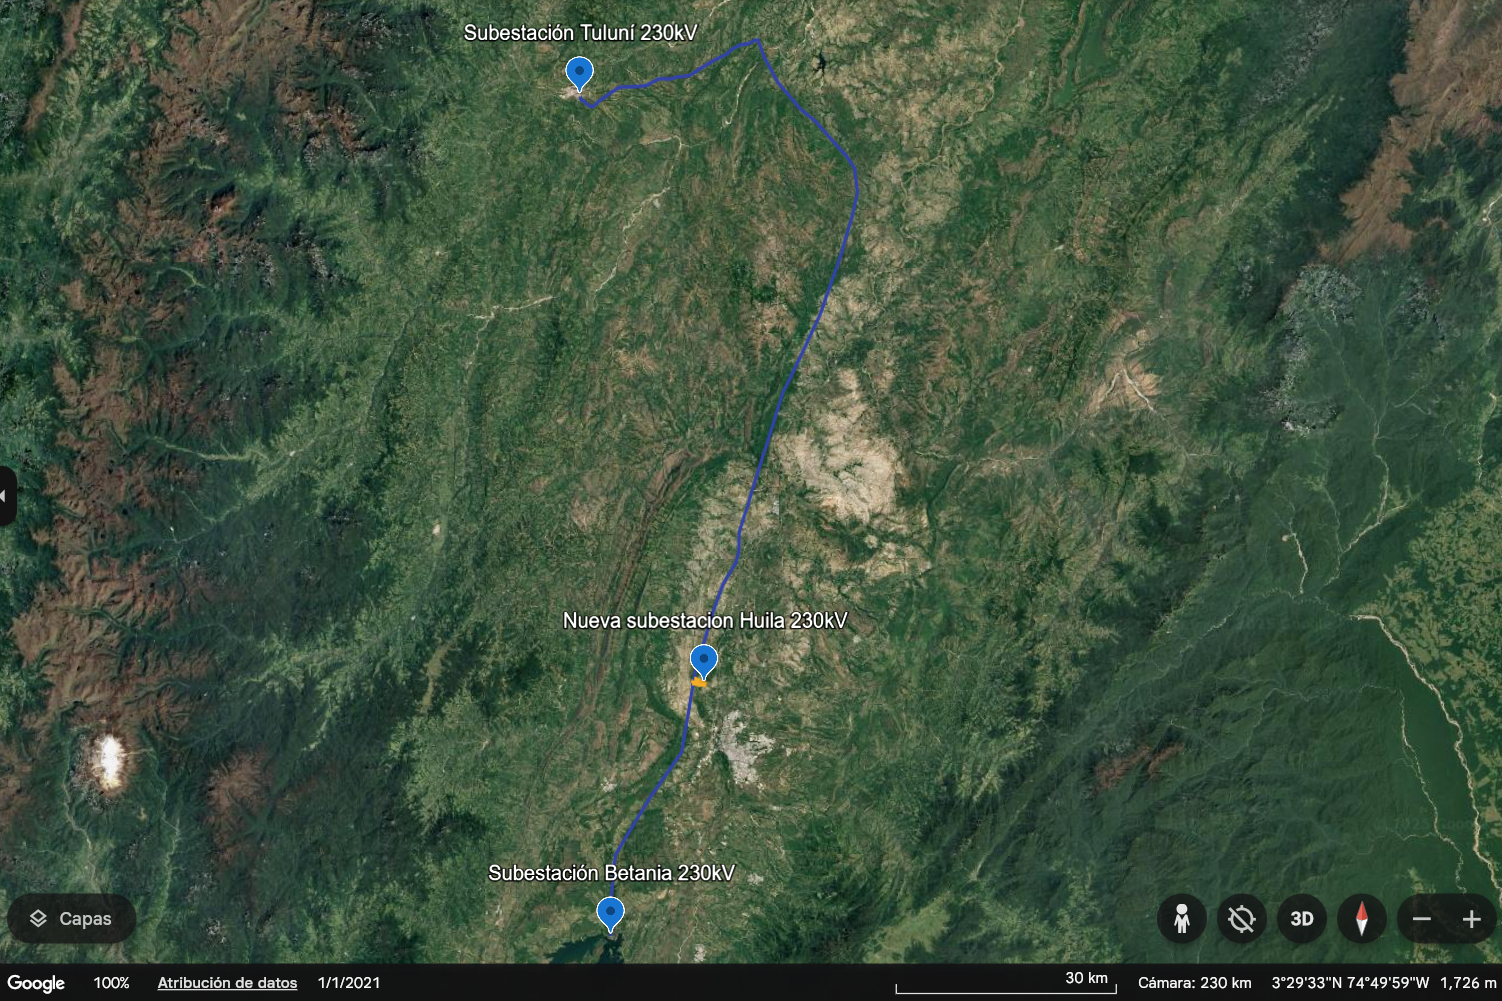
\includegraphics[width=1\textwidth]{1mer avance foticos/Huila 230kV - Google Earth - sin mirolindo.png}
        \caption{Nueva subestación huila conectada a la subestación Tuluní y Betania.} % Título de la figura
        \label{fig:sin mirolindo} % Etiqueta para referencias
    \end{subfigure}
    \begin{subfigure}{0.5\textwidth}
        \centering % Centra la imagen
        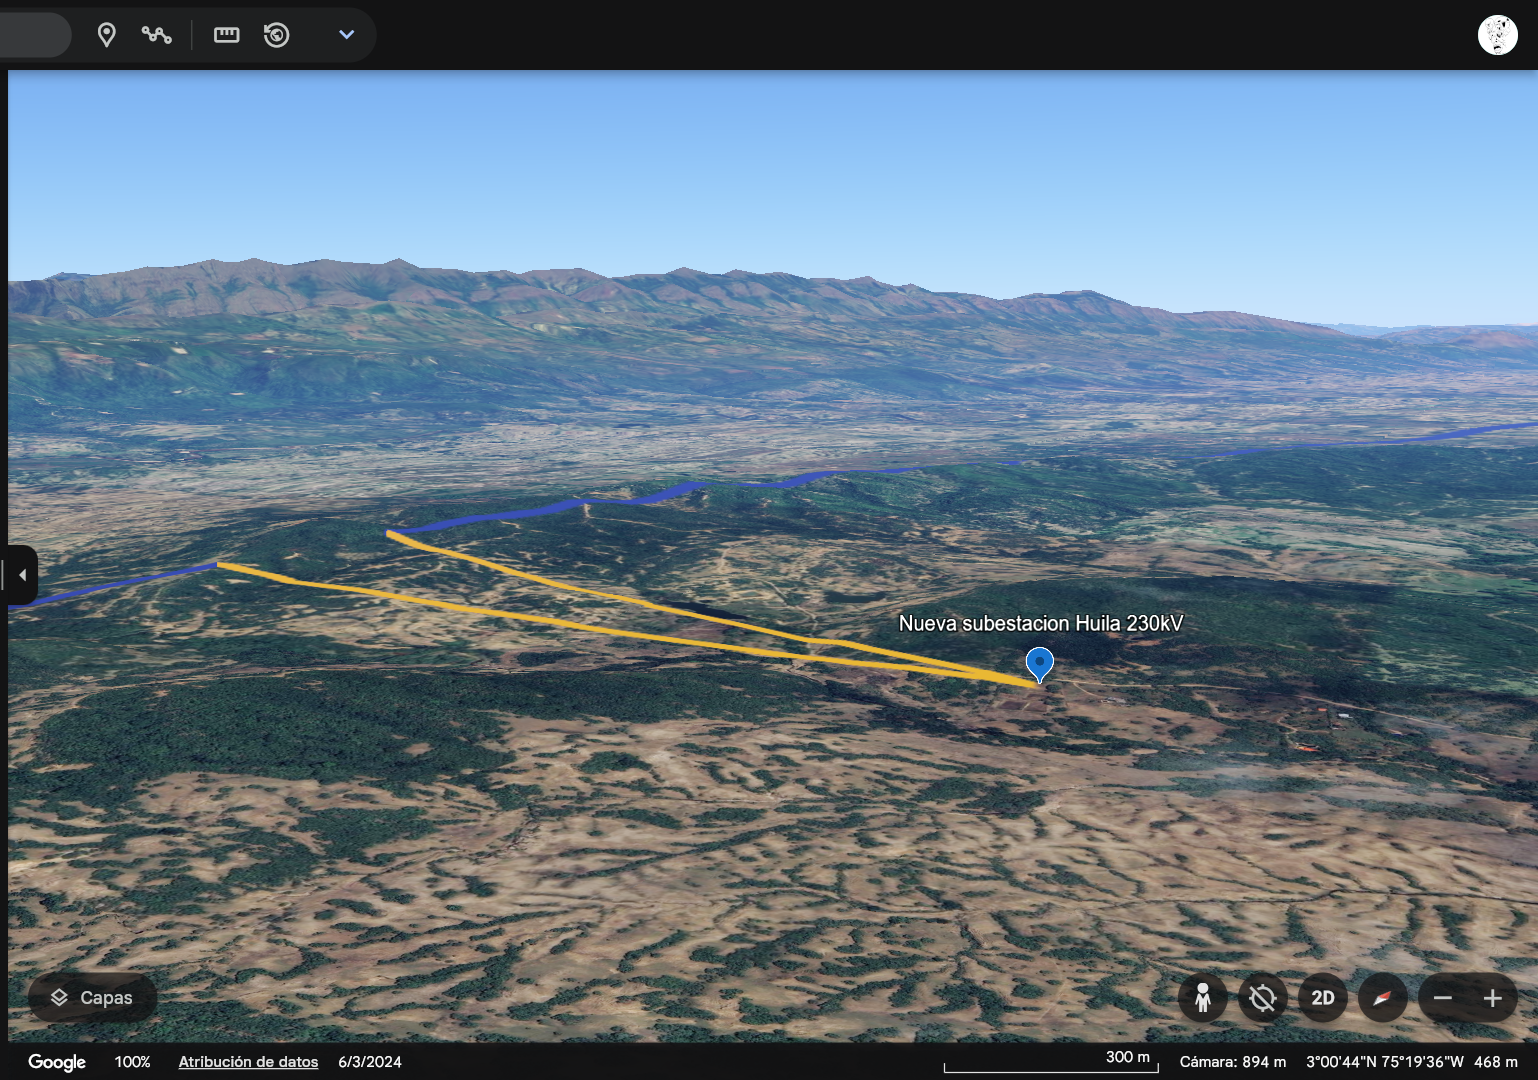
\includegraphics[width=1\textwidth]{1mer avance foticos/Huila 230kV - Google Earth - nueva acercada.png}
        \caption{Acercamiento a la nueva subestación huila conectada a la subestación Tuluní, Betania y Mirolindo.} % Título de la figura
        \label{fig:nueva acercada} % Etiqueta para referencias
    \end{subfigure}
\end{figure}


\begin{figure}[h!] % 'h' coloca la figura aquí
    \centering % Centra la imagen
    \begin{subfigure}{0.5\textwidth}
        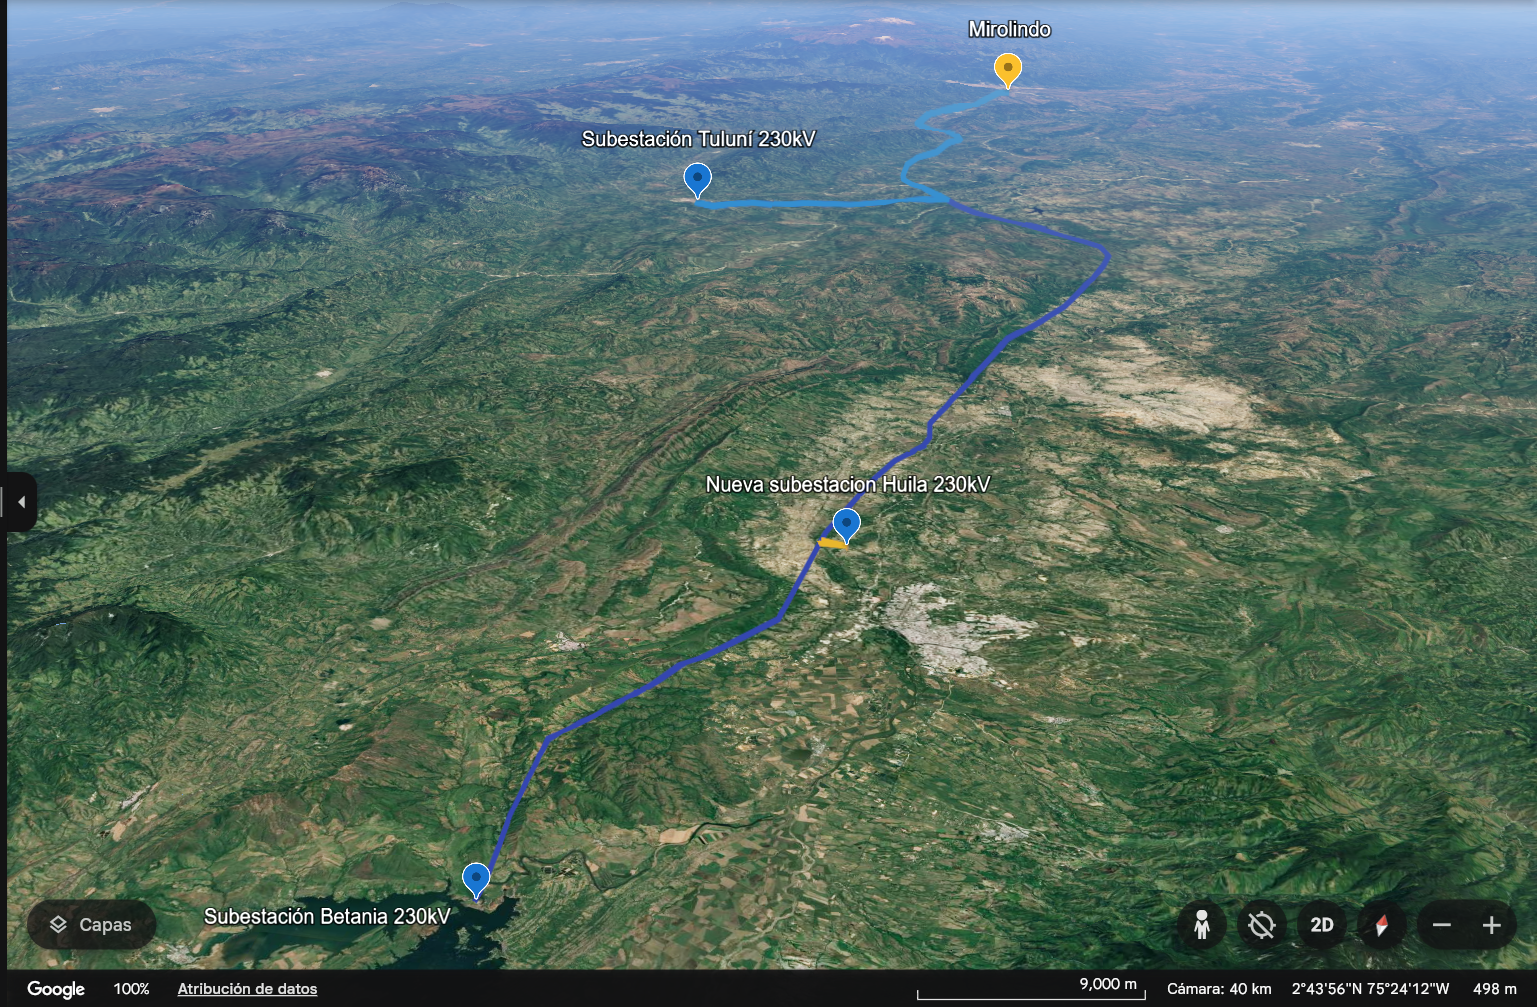
\includegraphics[width=1\textwidth]{1mer avance foticos/Huila 230kV - Google Earth - completo inclinado.png}
        \caption{Nueva subestación huila conectada a la subestación Tuluní, Betania y Mirolindo.} % Título de la figura
        \label{fig:todo angulo} % Etiqueta para referencias
    \end{subfigure}
    \hfill % Espacio horizontal entre las subfiguras
    \begin{subfigure}{0.5\textwidth}
        \centering % Centra la imagen
        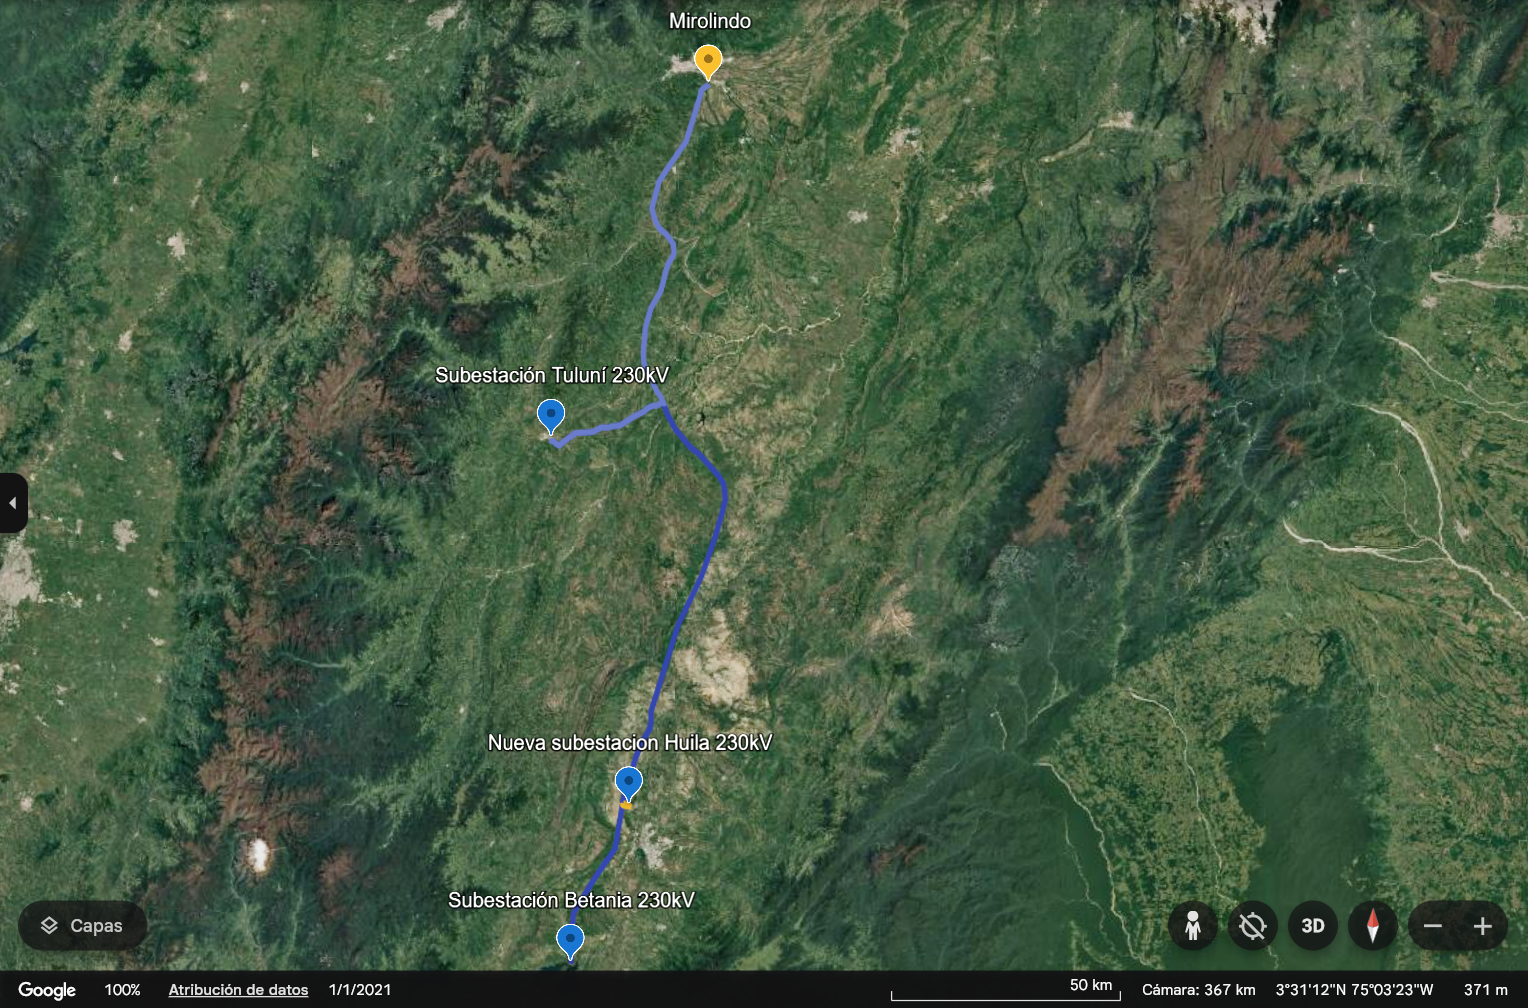
\includegraphics[width=1\textwidth]{1mer avance foticos/Huila 230kV - Google Earth - completo.png}
        \caption{Nueva subestación huila conectada a la subestación Tuluní, Betania y Mirolindo.} % Título de la figura
        \label{fig:todo} % Etiqueta para referencias
    \end{subfigure}
\end{figure}